\documentclass[12pt]{article}
\usepackage{spikey}
\usepackage{amsmath}
\usepackage{amssymb}
\usepackage{soul}
\usepackage{float}
\usepackage{graphicx}
\usepackage{hyperref}
\usepackage{xcolor}
\usepackage{chngcntr}
\usepackage{centernot}
\usepackage{datetime}
\usepackage[shortlabels]{enumitem}

% Set font.
\usepackage{fontspec}
 
\setmainfont{Times New Roman}
%\usepackage{mathptmx}
%\usepackage[MnSymbol]{mathspec}
%\setallmainfonts{Times New Roman}

\usepackage[margin=1truein]{geometry}
\usepackage{setspace}
\linespread{1.15}

\counterwithin{equation}{section}
\counterwithin{theorem}{section}
\counterwithin{lemma}{section}
\counterwithin{corollary}{section}
\counterwithin{proposition}{section}
\counterwithin{remark}{section}
\counterwithin{example}{section}
\counterwithin{definition}{section}

% Bib package
\usepackage{apacite}

\title{Title \footnote{Compile Date: \currenttime\ \today}}

\author{Tianyu Du \footnote{\texttt{tianyu.du@mail.utoronto.ca}}}

\begin{document}
	\maketitle
	\tableofcontents
	\newpage

	\section{Missing Data}
	\par
 
	\section{Day of the Week Effect}
	\par \cite{Hess1981}
	\par The following figures present distributions of crude oil returns computed using
	\begin{align}
		r_t &:= \ln(p_t) - \ln(p_{t - \Delta})
	\end{align}
	where $t - \Delta$ is the last trading day before day $t$. For instance, if $t$ is a Monday, then $r_t$ computes the crude oil return between the close price on Monday and the close price on Friday.
	\begin{figure}[H]
		\center
		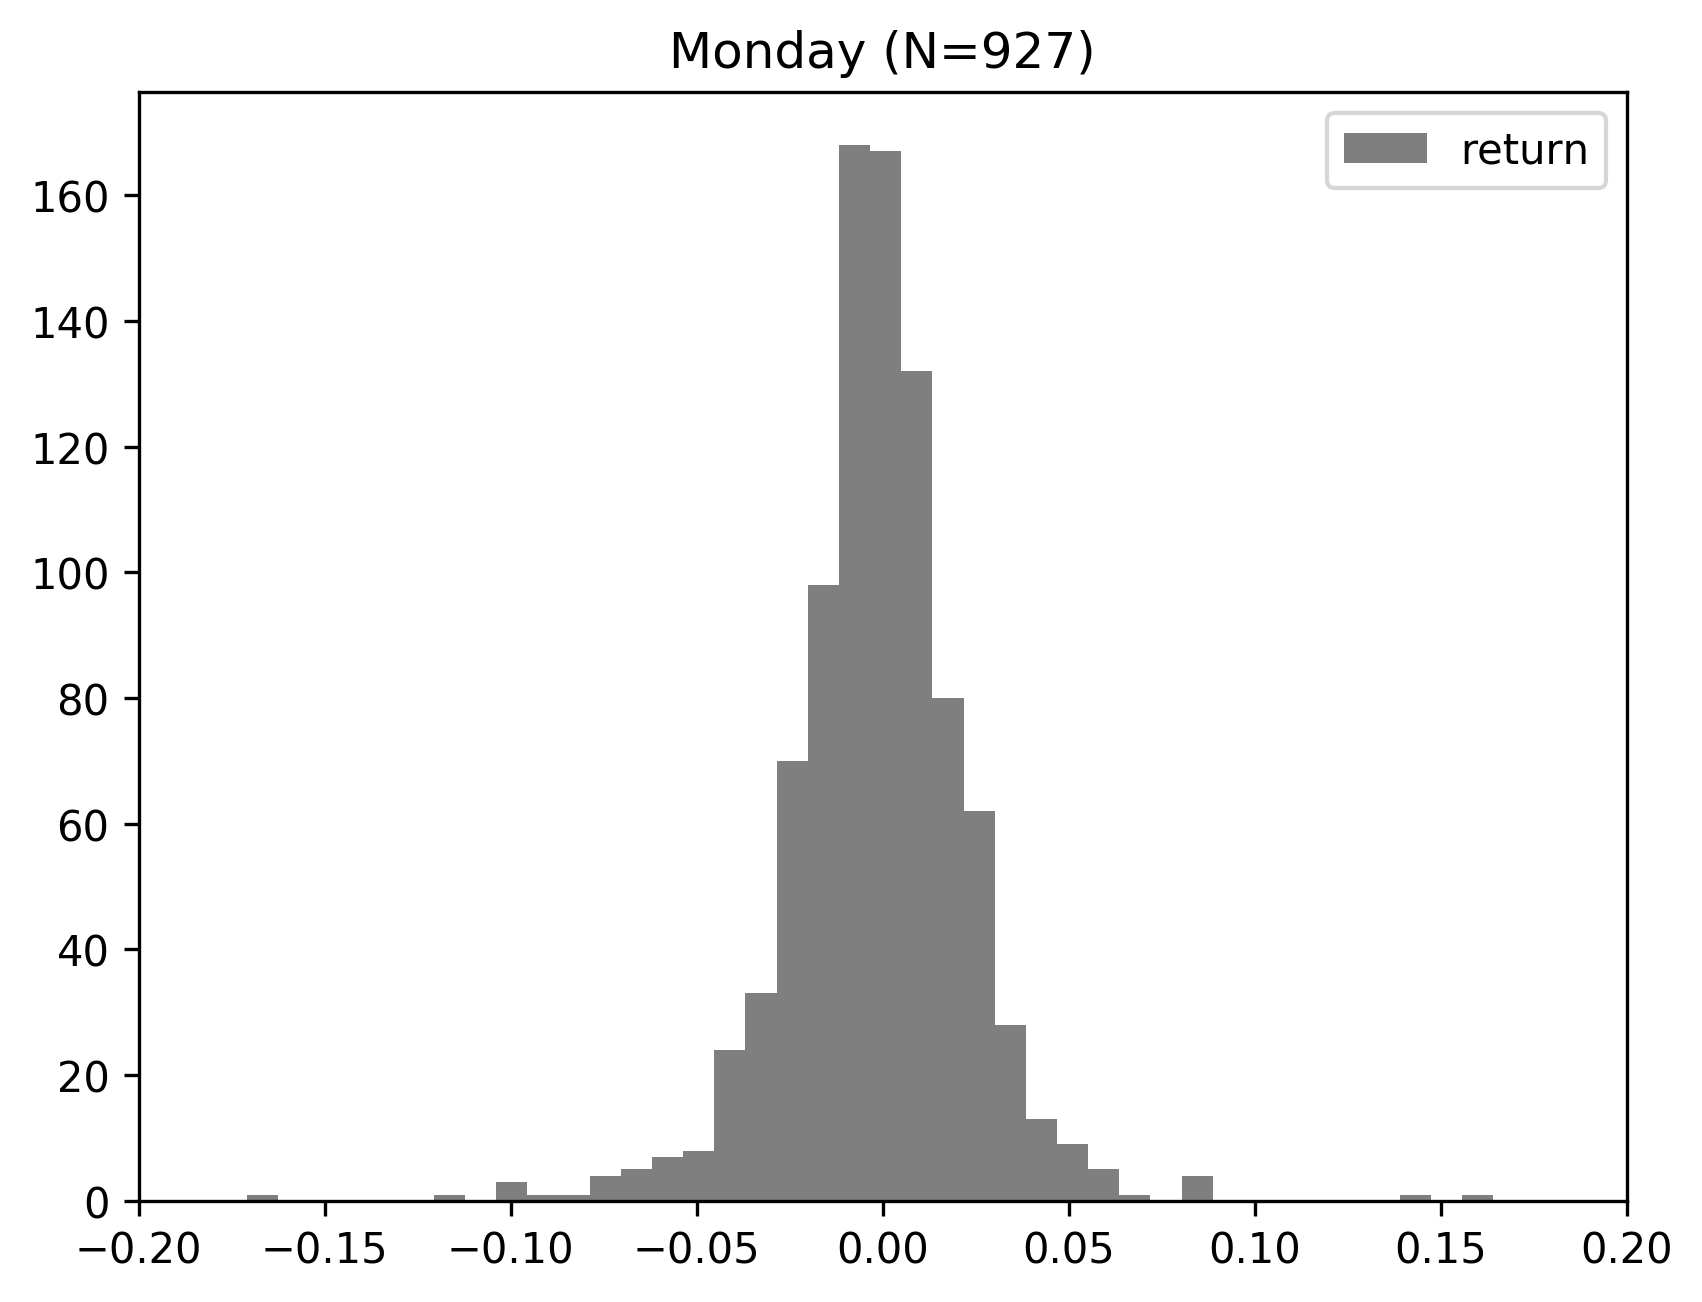
\includegraphics[width=0.45\linewidth]{figures/day_of_week_effect/dist_returns_Monday.png}
		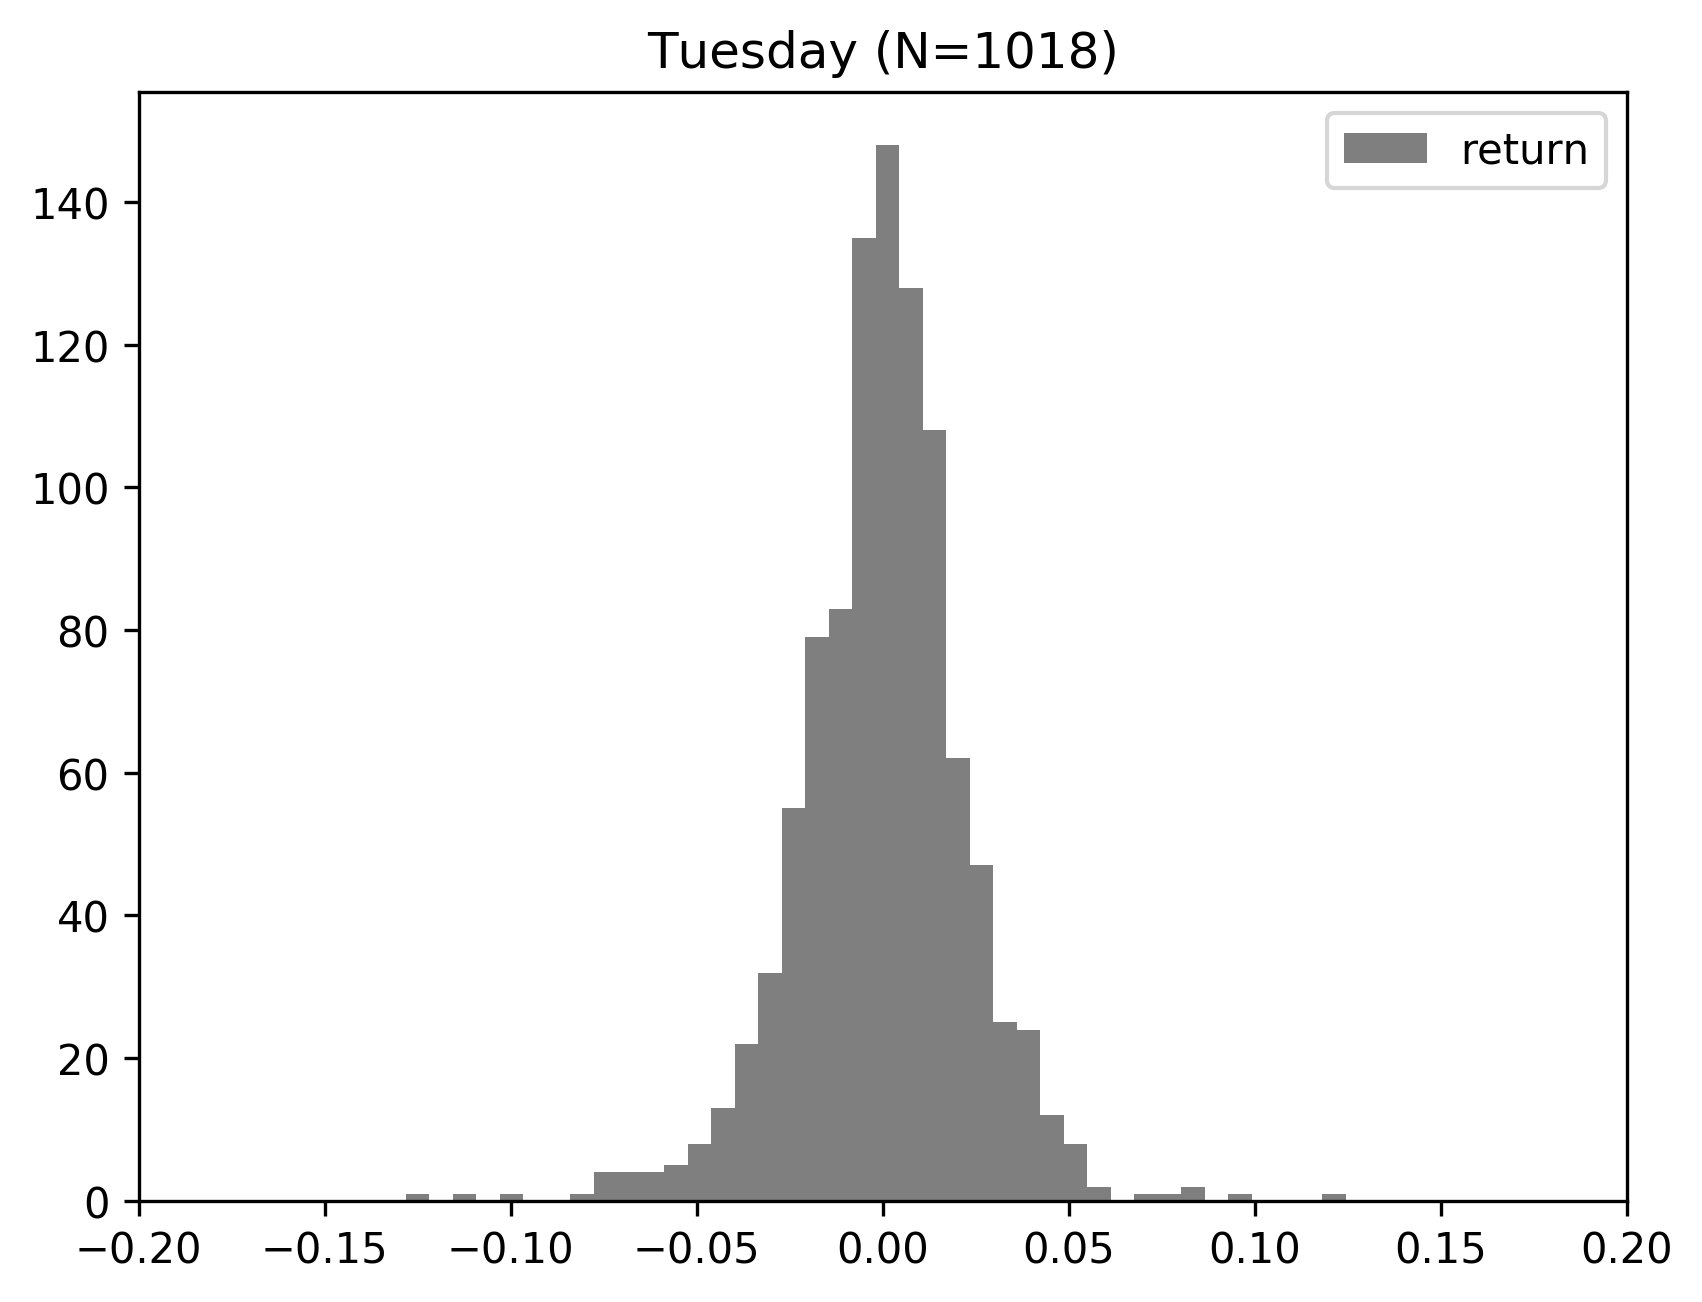
\includegraphics[width=0.45\linewidth]{figures/day_of_week_effect/dist_returns_Tuesday.png}
		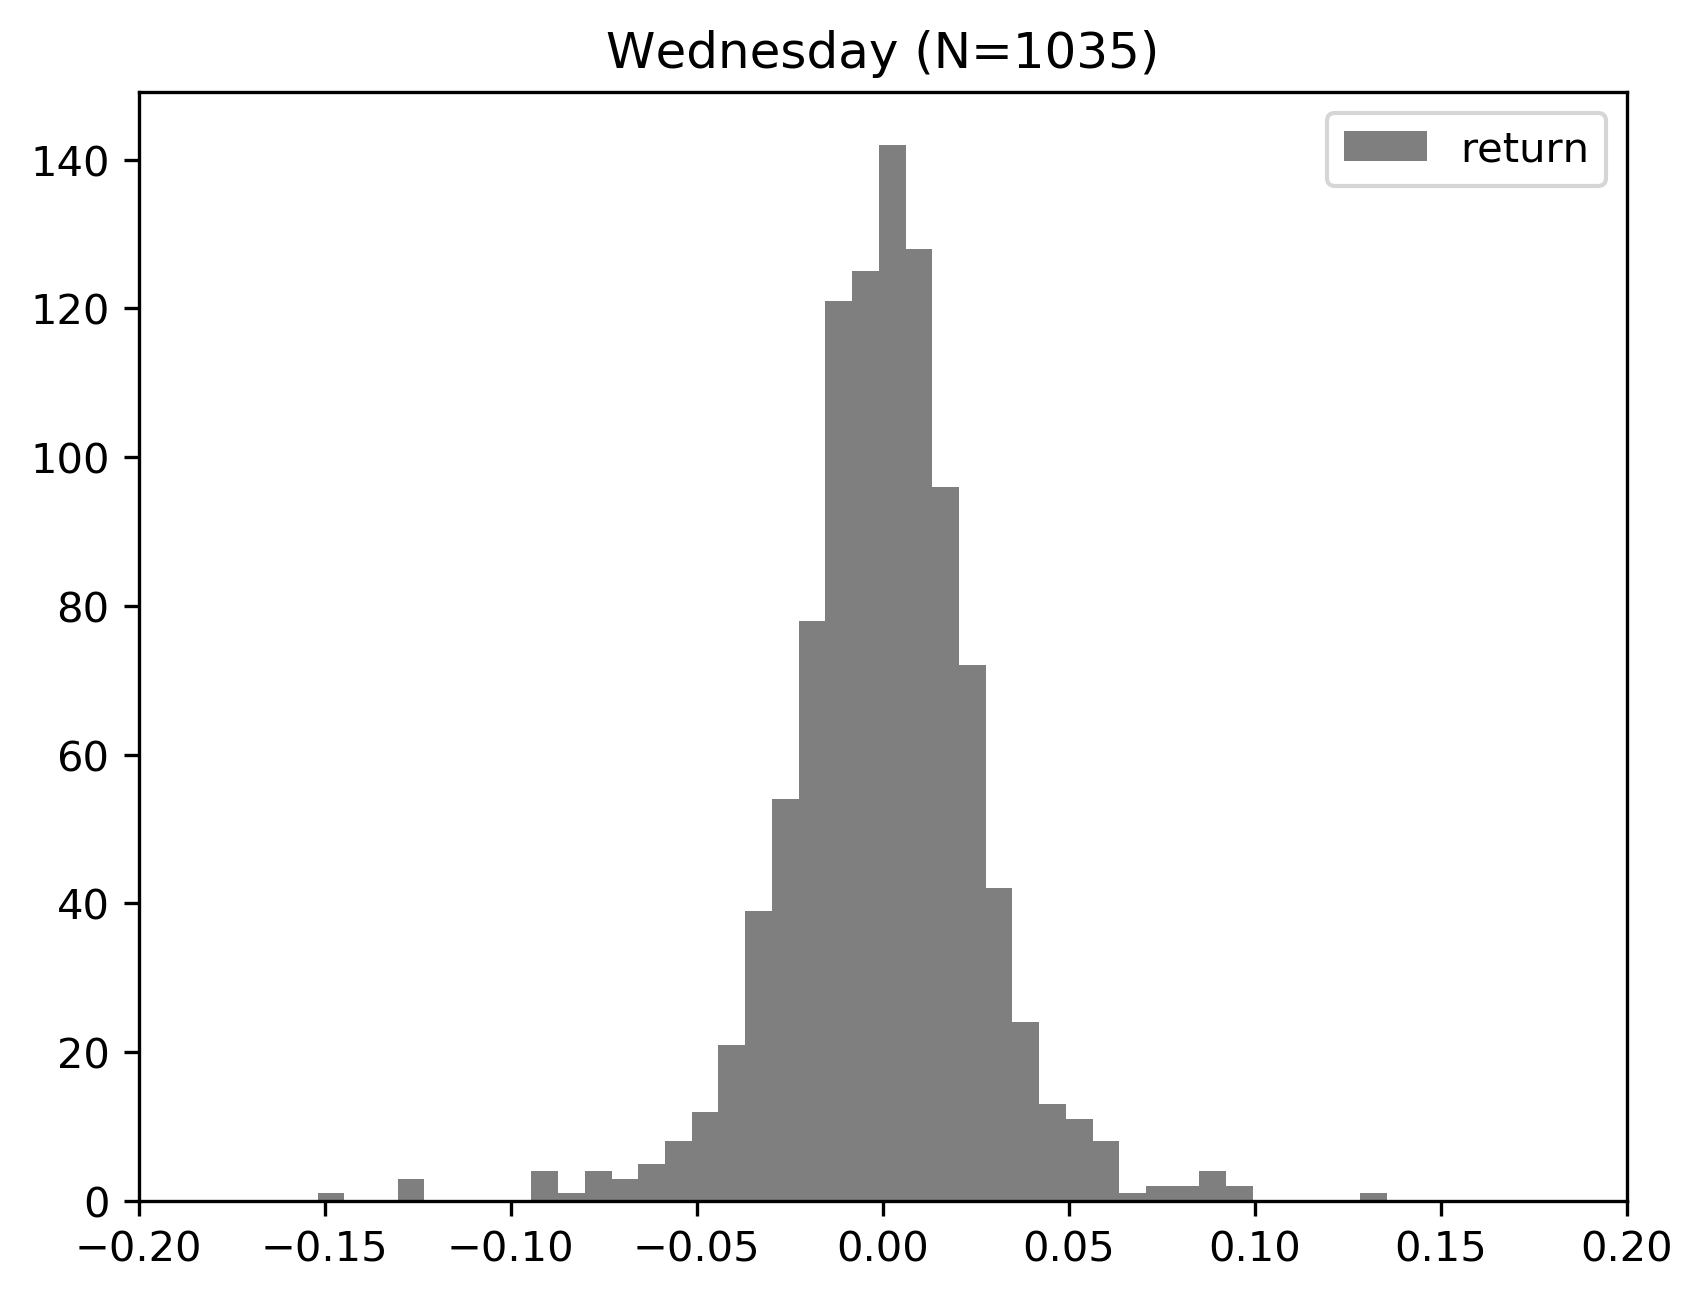
\includegraphics[width=0.45\linewidth]{figures/day_of_week_effect/dist_returns_Wednesday.png}
		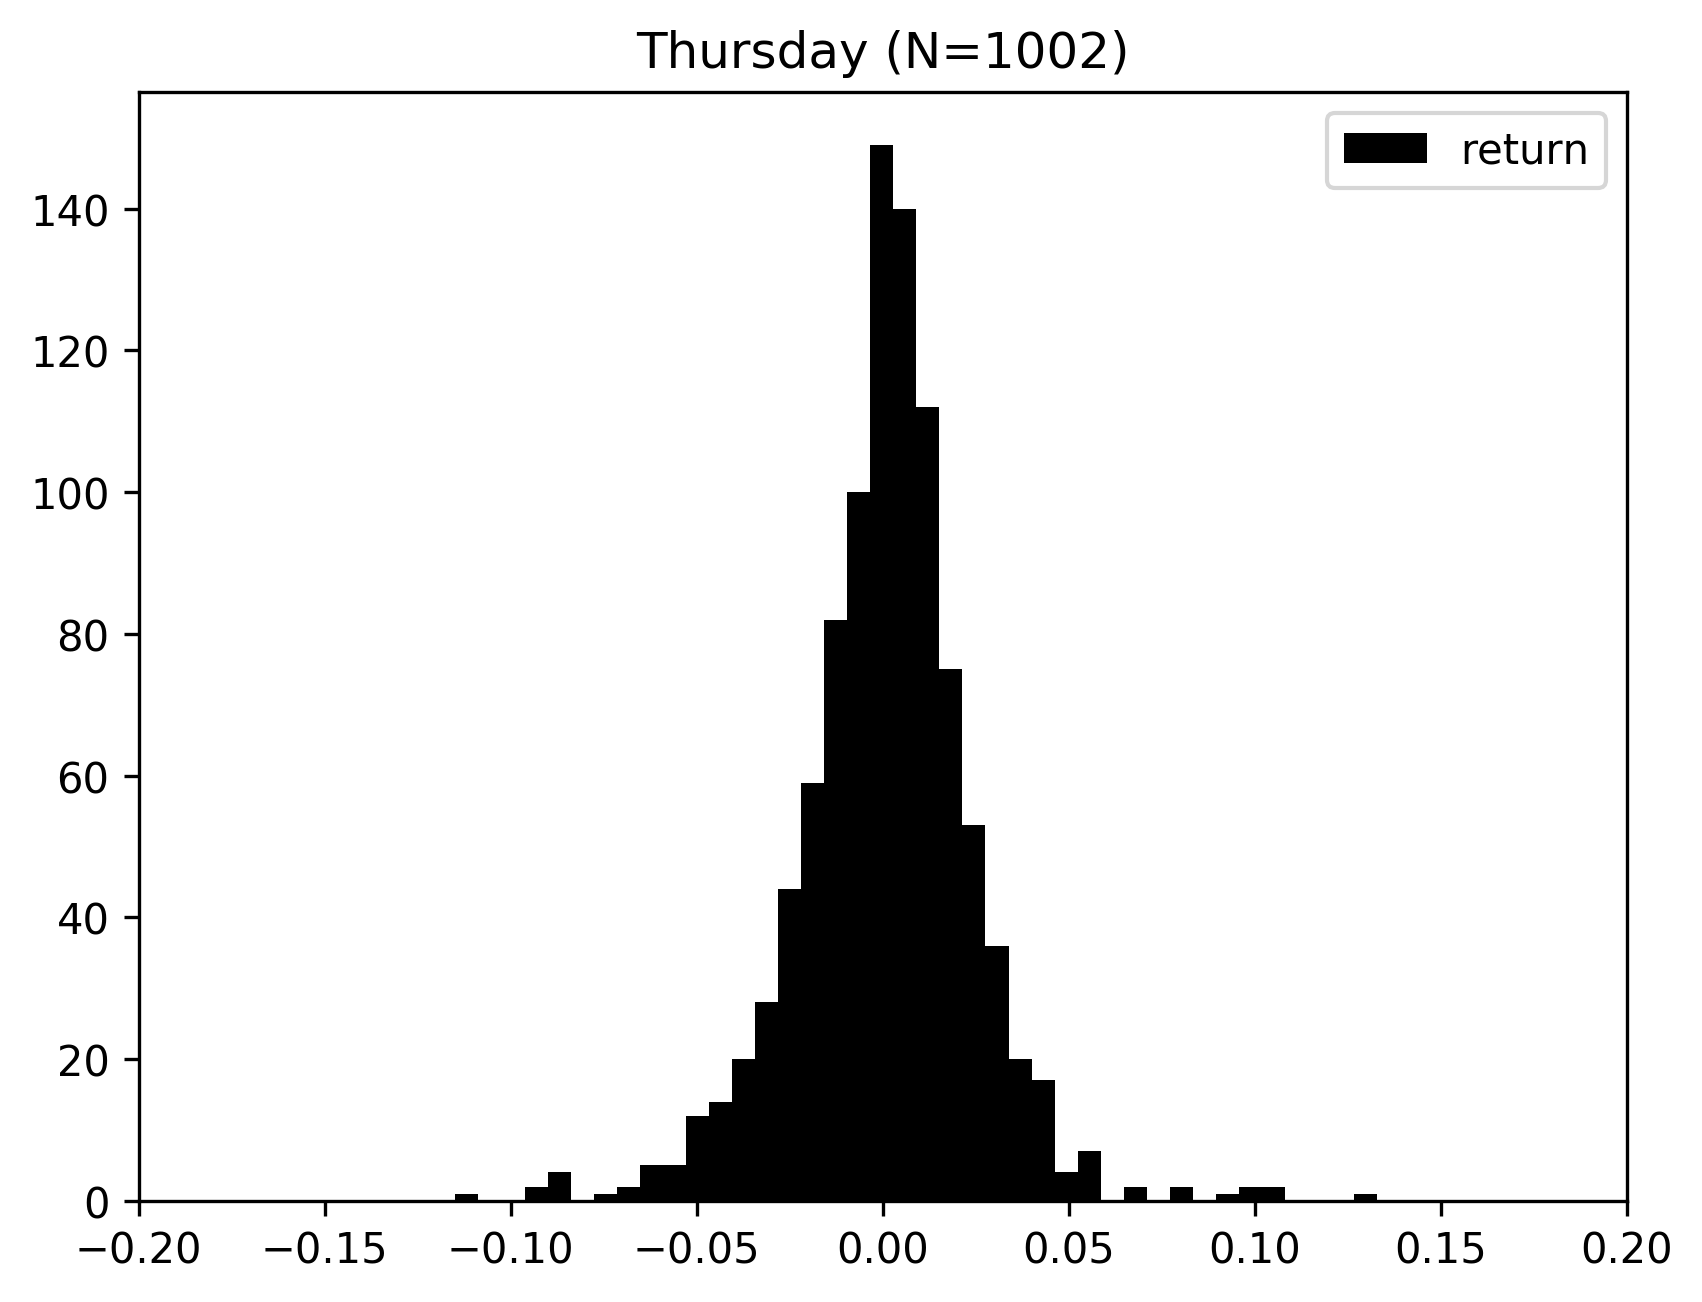
\includegraphics[width=0.45\linewidth]{figures/day_of_week_effect/dist_returns_Thursday.png}
		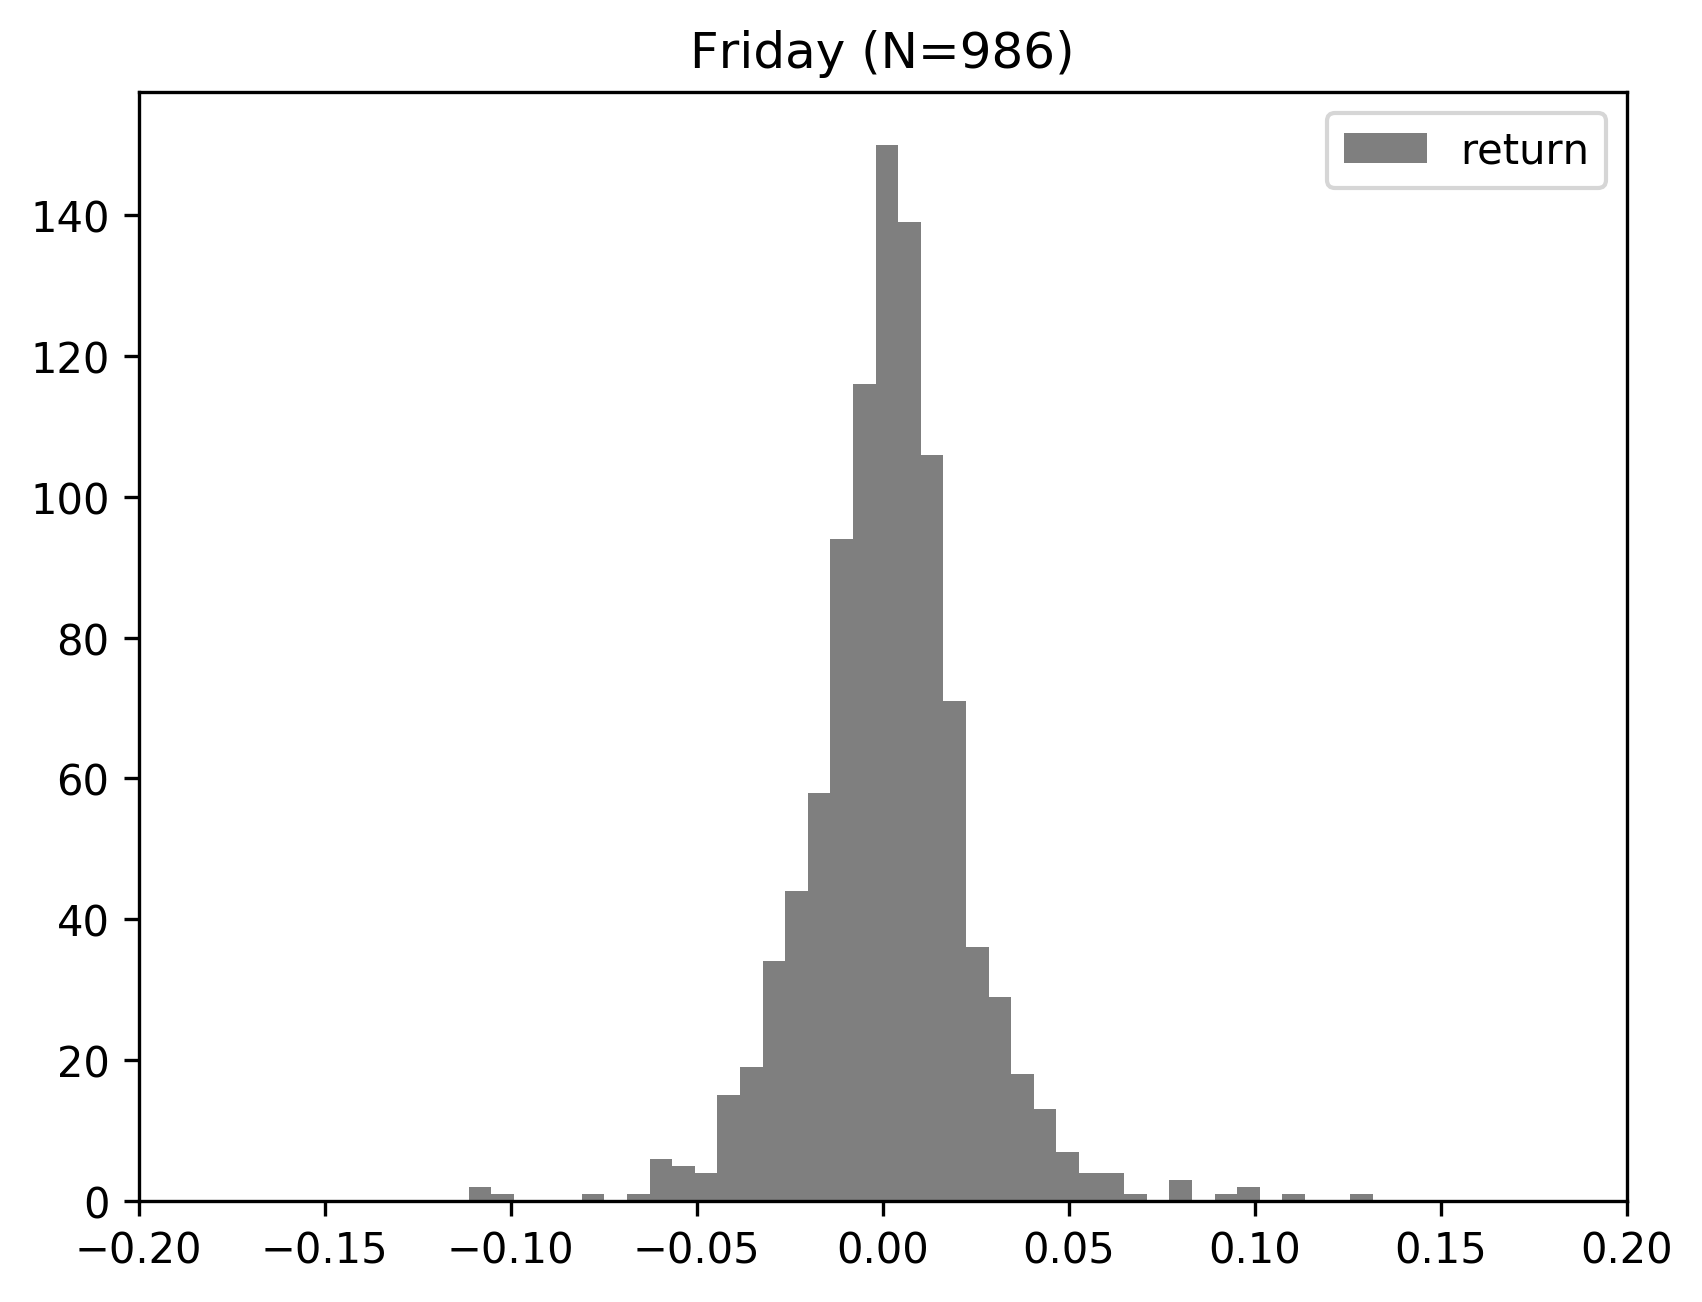
\includegraphics[width=0.45\linewidth]{figures/day_of_week_effect/dist_returns_Friday.png}
		\caption{Crude oil returns on each weekday. Weekend data are not available in the daily dataset provided by EIA. The range of y-axis in all five histograms are from -0.2 to 0.2. $N$s in parentheses denote the number of observations. See appendix for distributions of crude oil prices.}
	\end{figure}

	\begin{table}[H]
		\small
		\center
		\begin{tabular}{|l|c c c c|}
			\hline
			Day of the week & Num. Obs. & Mean & Std. & $3^{rd}$ Moment \\
			\hline
			Monday & 927 & 62.072 & 26.493 & 7081.163 \\
			Tuesday & 1019 & 61.828 & 26.317 & 6895.638 \\
			Wednesday & 1022 & 61.810 & 26.398 & 7049.810 \\
			Thursday & 1002 & 62.005 & 26.431 & 6955.555 \\
			Friday & 986 & 62.079 & 26.247 & 6676.566 \\
			\hline
		\end{tabular}
		\caption{Summary statistics of crude oil prices on each day of week}
	\end{table}

	\begin{table}[H]
		\small
		\center
		\begin{tabular}{|l|c c c c|}
			\hline
			Day of the week & Num. Obs. & Mean & Std. & $3^{rd}$ Moment \\
			\hline
			Monday & 927 & -0.002 & 0.025 & -0.0000019 \\
			Tuesday & 1018 & -0.000 & 0.023 & -0.0000031 \\
			Wednesday & 1022 & 0.000 & 0.027 & -0.0000054 \\
			Thursday & 1002 & 0.001 & 0.024 & -0.0000006 \\
			Friday & 986 & 0.002 & 0.023 & 0.0000021 \\
			\hline
		\end{tabular}
		\caption{Summary statistics of crude oil returns on each day of week. The first day (January 1, 2000) of the oil price dataset was Saturday, and the observation on the following Monday (January 3) was missing. Hence, the return on Tuesday (January 4) could not be computed because it was the first trading day in this dataset, and there are only 1018 Tuesday in the dataset of returns.}
	\end{table}
	
	\subsection{Kolmogorov-Smirnov test for Distributional Similarities}
	\par Smirnov developed a non-parametric method of testing the equality between two continuous distributions, with CDFs $F(x)$ and $G(x)$ respectively, \cite{Smirnov1939}. Refer to Hodges' work for a detailed review on the Kolmogorov-Smirnov test \cite{Hodges1957}. Given two datasets, say returns on Monday and Tuesday, the null hypothesis says those two datasets are drawn from the same distribution, and the alternative says they are from different distributions \footnote{Different alternative hypotheses can be used in Kolmogorov–Smirnov test: i) $H_1: F(x) \geq G(x)$, ii) $H_1: F(x) \leq G(x)$, and iii) $H_1: F(x) \neq G(x)$. This paper is using the third (two-tailed) alternative hypothesis.}.
	Firstly, the Kolmogorov–Smirnov test constructs the empirical CDFs $F_{Mon, 927}(x)$ and $F_{Tue, 1018}(x)$ from the dataset. Then, the Kolmogorov–Smirnov statistic measures the maximum discrepancy between two distribution functions, which is
	\begin{align}
		D := \sup_x \abs{F_{Mon, 927}(x) - F_{Tue, 1018}(x)} \in [0, 1]
	\end{align}
	A smaller $D$-statistic implies stronger distributional similarity between two distributions. For example, when $F_{Mon, 927}(x)$ and $F_{Tue, 1018}(x)$ are exactly the same, the $D$-statistic is zero. In contrast, let $X=0$ and $Y=1$ be two deterministic random variables, in this case, $D_{X, Y} = 1$.
	\begin{table}[H]
		\small
		\center
		\begin{tabular}{|l|c|c|c|c|c|}
			\hline
			$D$-Statistic ($P$-Value)& Monday & Tuesday & Wednesday & Thursday & Friday \\
			\hline 
			Monday    & 0.000 (1.000) & \textbf{0.061 (0.048)} & \textbf{0.065 (0.030)} & \textbf{0.092 (0.001)} & \textbf{0.092 (0.001)} \\
			Tuesday   &               & 0.000 (1.000) & \textbf{0.044 (0.260)} & 0.036 (0.505) & 0.044 (0.264) \\
			Wednesday &               &               & 0.000 (1.000) & 0.053 (0.114) & \textbf{0.073 (0.009)} \\
			Thursday  &               &               &               & 0.000 (1.000) & 0.025 (0.900) \\
			Friday    &               &               &               &               & 0.000 (1.000) \\
			\hline
		\end{tabular}
		\caption{The Kolmogorov-Smirnov $D$-Statistic for all pairs of distributions. Bold font indicates the null hypothesis is rejected at a significance level of 0.05, which implies discrepancy in distributions.}
	\end{table}
	\hl{The table above} presents the Kolmogorov-Smirnov $D$-Statistic for distributions of every pairs of days. At a significance level of 0.05, we can see that Monday follows a distribution significantly different from distributions other days follow. Because the dataset does not contain weekend data, the return on Monday is always computed using the difference between log prices on Monday and the previous Friday (Thursday if Friday is not a trading day and so on). Therefore, returns associated with Mondays pick the so-called weekend effect.


	% Bib
	\bibliographystyle{apacite}
	
	\bibliography{thesis.bib}

	\section{Appendix}

\end{document}






















